\chapter{Computing Fundamentals in LabVIEW}
In this chapter, we will go over some of the basic building blocks of a computer program in the context of $\labview$. This chapter will be heavy on examples in $\labview$, but will be light on the trivial details such as how to open a VI and how to place functions and controls. If you have not already done so, review the exercise in section \ref{HowToPlace} in Chapter 1.\\

If you get stuck, you may open the $\labview$ help files my pressing \texttt{Ctrl+?} and navigating to the ``Fundamentals'' section. If you would like to see more examples of how things are done in $\labview$, on the taskbar select ``Help'' and navigate down the menu to find ``Find Examples...'', here you will find a library of examples. These examples range from trivial arithmetic, to programs which would make you a cup of coffee if you supply it with enough hardware.

\section{Decision making structures}
Without the ability to make decisions, computers would not be as useful as they are now. Try to think of a computer program that makes no decisions based on it's input, they do exist and some are even useful. We are not interested in such academic programs, we want our computer to do the heavy lifting for us, just imagine clicking \texttt{yes} or \texttt{no} for a data set of a billion numbers. My computer can do that in $5.76$ seconds (I just checked using $\labview$).\\

If you are familiar with programming, you know that the most fundamental decision making block is an ``if-statement''. You supply the block with a condition, and the program executes statements based on that condition. Technically speaking, $\labview$ has no such thing as an if-statement, it has ``case-structures'' and ``ternary-operators''.

\subsection{Case Structures}
The case structure executes a block of code according to its input condition. In $\labview$, the input condition may be either a boolean value, an enumeration, or an error value. Figure \ref{ch2egTrue} (A) shows how a case structure looks, a thick grey box with a green \texttt{?} and a selection box stating ``True''. What ever is inside this grey box will be executed if a boolean true value is wired into the conditional terminal, the green \texttt{?}. Figure \ref{ch2egFalse} shows what would be executed if the condition is false.\\
\begin{figure}
	\centering
	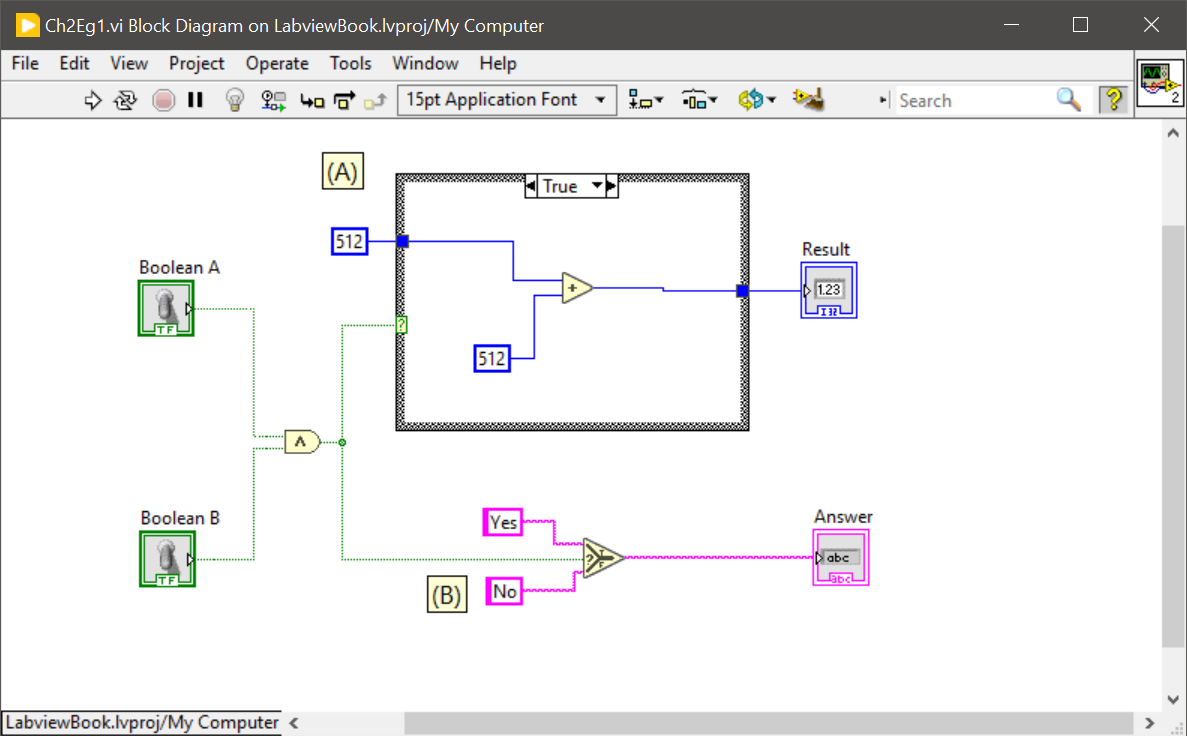
\includegraphics[width=\textwidth]{ch2eg1True}
	\caption{A case structure showing its truth block (A), and a ternary operator (B).}
	\label{ch2egTrue}
\end{figure}
\begin{figure}
	\centering
	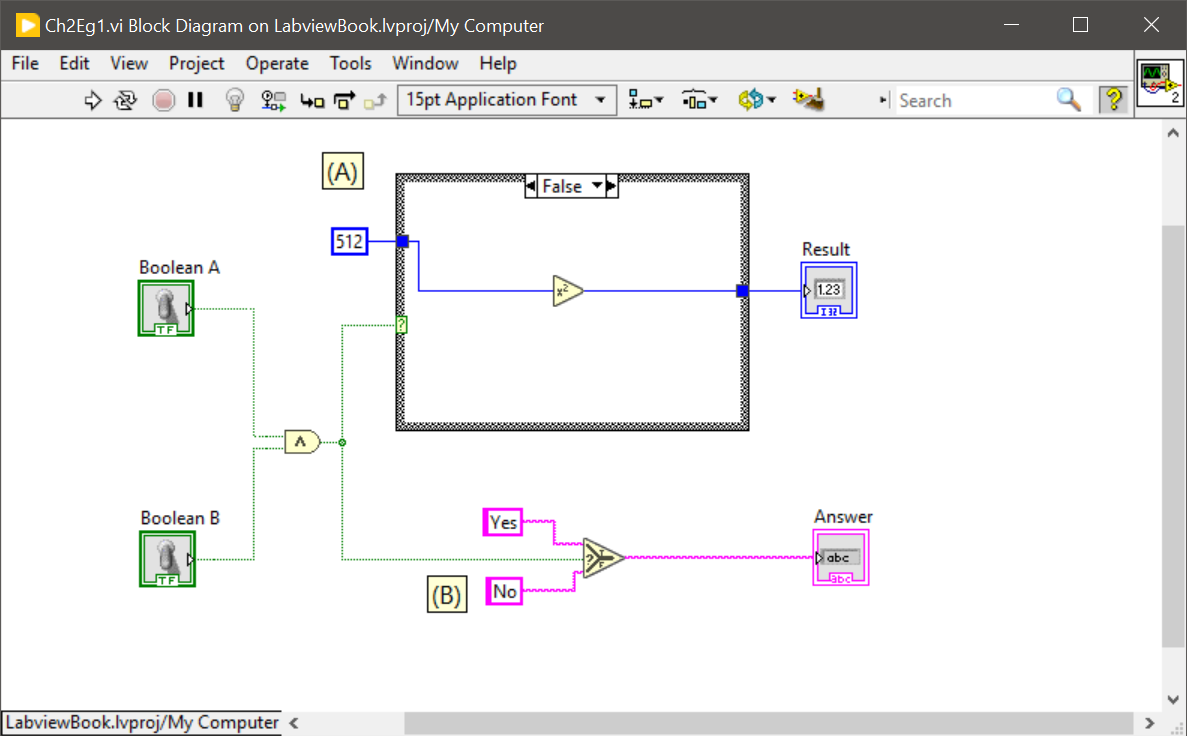
\includegraphics[width=\textwidth]{ch2eg1False}
\caption{A case structure showing its false block (A), and a ternary operator (B).}
\label{ch2egFalse}
\end{figure}

Comparison functions in $\labview$ produce only boolean values, this you have seen in the examples so far. Feeding these boolean values into case structures allow you to select different operations to be preformed. The example provided in figures \ref{ch2egTrue} \& \ref{ch2egFalse} show how you would choose two different operations on an integer. If the condition is true, 512 is added to the input number and the result is given, the indicator outside the case structure.  If the value is false, 512 is squared and the result given.\\

A case structure also accepts enumeration values. This is similar to a switch structure in \texttt{C} programming. In figure \ref{ch2eg2}, a value named ``Multiply'' is placed into the case structure. This allows you to have many paths of execution in a single structure. In the example, a simple calculator is made which takes two input numbers and an enumeration condition, the block then executes the proper logic and hands you the result at the end. One of the mini projects at the end of this chapter will require you to create a 4-function calculator.\\
\begin{figure}
	\centering
	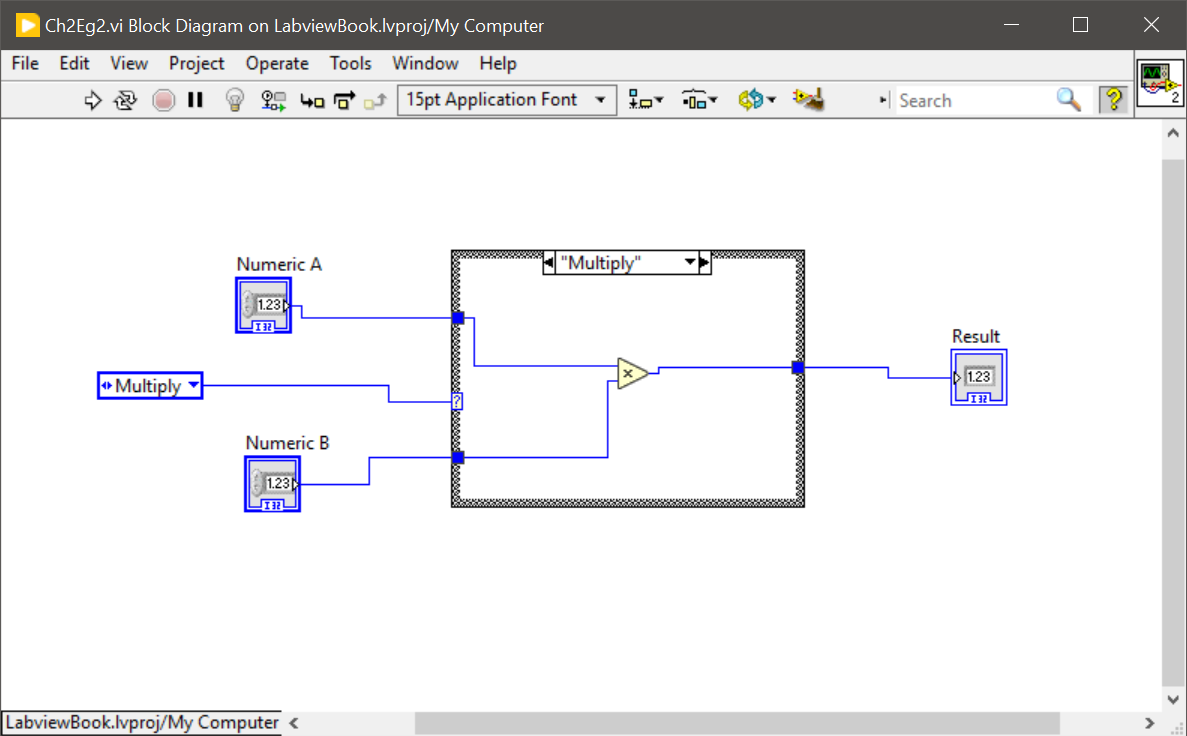
\includegraphics[width=\textwidth]{ch2eg2}
\caption{A simple calculator using an enumeration type and a case structure.}
\label{ch2eg2}
\end{figure}

\subsection{Ternary operators}
The plural in the title is misleading, there is only one ternary operator in $\labview$. Figure \ref{ch2egTrue} (B), on page \pageref{ch2egTrue}, is this little function in action. You supply it with a boolean value and outputs either its truth or false value. In this example, if the boolean value is true, then the ternary operator outputs the string ``Yes''.\\

The only caveat is that you must use the same variable type for its true and false inputs, this type will also be its output type.  There really isn't anything more special about the ternary operator. It is possible to implement a ternary operator using a case structure, an exercise left for the reader.

\section{Code looping structures}
In the previous section, I mentioned that my computer could make a billion decisions in $5.76$ seconds. The program certainly did not contain a billion case structures, it only had one.\\

It is quite rare for a program to only make one decision before execution stops, most probably you have a few decisions which would need to be repeated thousands of times per execution. One may even say that you would like to have a program perform a ``loop'' of decisions. This is were loop structures come into play.\\

The two loop structures available to us in $\labview$ is the ``For Loop'' and the ``While Loop''. The for loop executes a set number of times while the while loop executes until some specified condition is met. These two structures are closely related however since the for loop can pretend to be a while loop. It is also worth mentioning in passing, to those of you with previous programming experience, that both loops act as `do-while'' loops since they execute at least once before evaluating their conditional terminals.\\

The flow of information in $\labview$ is rather unconventional, this will be elaborated upon in a future section, but for now there will be references to arrays, time functions, and shift registers without going into depth for either topics.

\subsection{For Loops}
A for loop executes a predetermined amount of times. Figure \ref{ch2eg3} is perhaps the most simple, yet interesting, loop possible in $\labview$. You set the number of times the loop should run in the ``Number of times'' control and the loop shows you the iteration step number along with a random floating point number between 0 \& 1. The little watch function in the bottom right corner is to slow the loop execution speed to twice every second so you are able to observe the number generated.\\
\begin{figure}
	\centering
	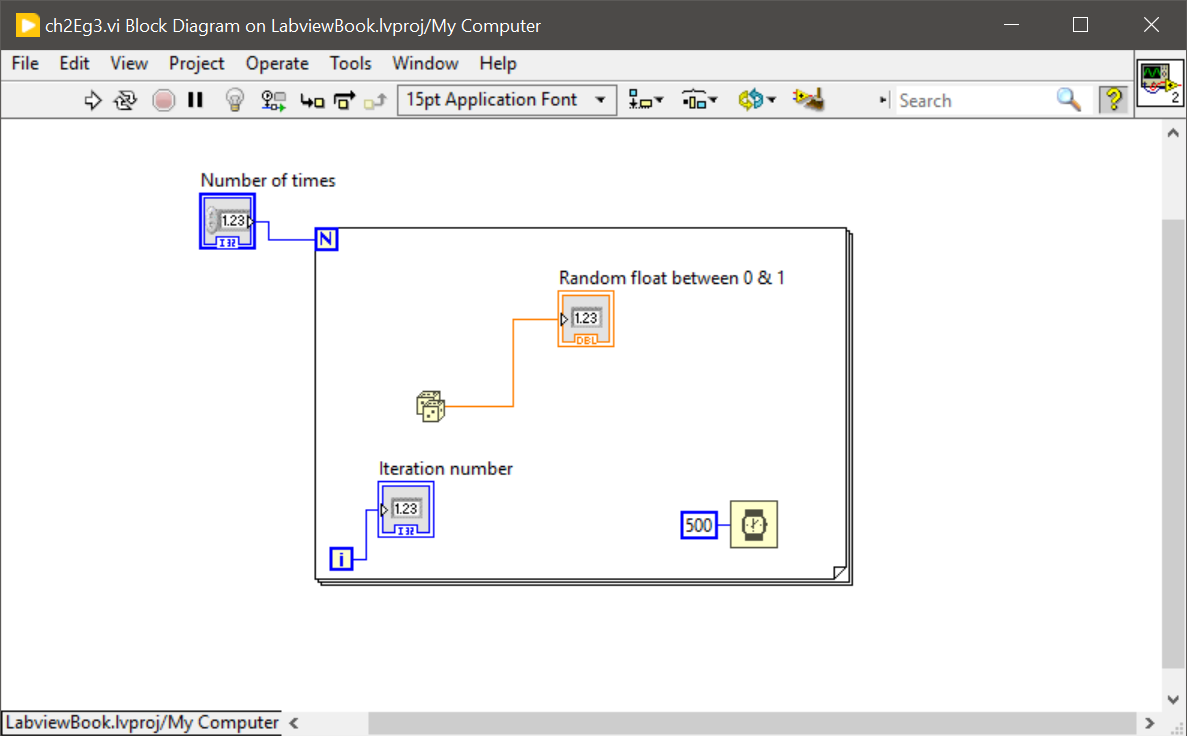
\includegraphics[width=\textwidth]{ch2eg3}
	\caption{A simple loop that ejects random numbers, two every second.}
	\label{ch2eg3}
\end{figure}

The example is heavily constrained however, there is no way for the information generated to be stored in memory so there is no knowlage for what the random number was in the previous iteration let alone what the series of generated numbers were.\\

Just by introducing a concept known as a shift register, we can actually start making useful programs, or what ever useful means in this case. A shift register allows you to store a variable from a current loop iteration so that it is useable in the next iteration. To illustrate this, let us create a loop that prints out, in sequence, the first 10 numbers in the Fibonacci sequence.\\

The Fibonacci sequence, defined by the recurrence relation:
\begin{equation*}
	F_0=0,\quad F_1=1,\quad F_n= F_{n-1} + F_{n-2}
\end{equation*}
An implementation of this may be found in figure \ref{ch2eg4}. On the right hand side of the loop structure is a little blue arrow in a box, this is the terminal where you value the number you want available to the next loop iteration. To add a shift register to a loop, \texttt{right click} on any side of the loop frame and select ``Add Shift Register'' from the drop-down menu.\\
\begin{figure}
	\centering
	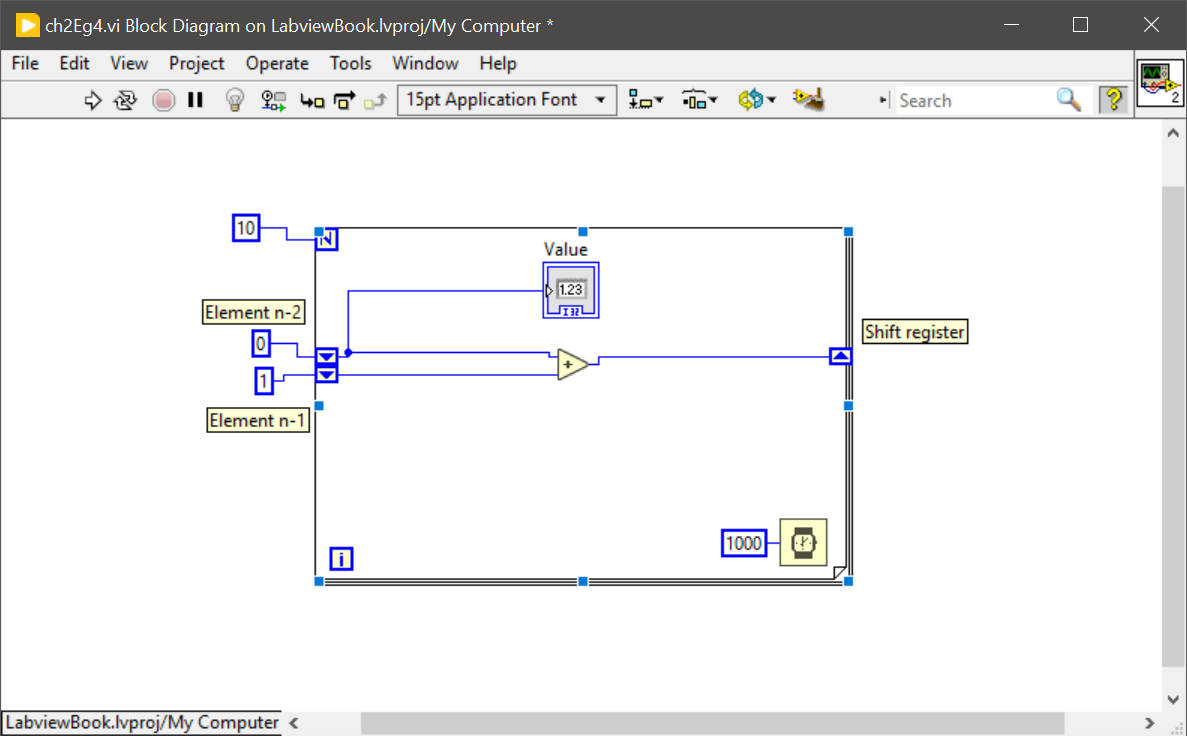
\includegraphics[width=\textwidth]{ch2eg4}
	\caption{A loop that displays the Fibonacci numbers, updating every second.}
	\label{ch2eg4}
\end{figure}

You may notice in that example that the left hand side has two little arrows stacked on top of each other, this gives you access to the previous iteration values. In this case the top arrow is the value of iteration n-2 and the bottom arrow is the value of iteration n-1. You can extend or reduce the number of iterations available by clicking and dragging the bottom edges of the shift register.\\

The values feeding into the left of the shift registers initialise the two first numbers in the sequence. If you do not do this, the two initial numbers would be $0$. Do not rely on such implicit details, if you want to have the first numbers to be $0$, wire in a zero constant explicitly. This will also show your intent in the code and not leave people reading the code guessing.\\

The indicator wired to the little blue \texttt{i} gives you access to the current iteration, starting from $0$ end ending in $n-1$. You don't need to memorise this, just hover your mouse over the little blue \texttt{i} and it will tell you. Although not exactly useful in this example, it makes working with arrays significantly easier so you should look forward to that.\\

\subsection{While Loops}
Suppose your program needs to monitor a temperature sensor and it requires the temperature to be above some set point before it turns on a fan, say. You can not know when this temperature threshold is reached, if it is ever ever reached. In such a case, a while loop allows us to execute some code only leaving the loop once some condition is met. If the condition is never met, then the loop never ends.\\

Figure \ref{ch2eg5} is the previous Fibonacci sequence program modified to use a while loop instead. Gone is the little blue \texttt{N} in the top left corner of the loop. Instead, a little red octagon is present at the bottom right corner of the loop. This is the conditional terminal\\
\begin{figure}
	\centering
	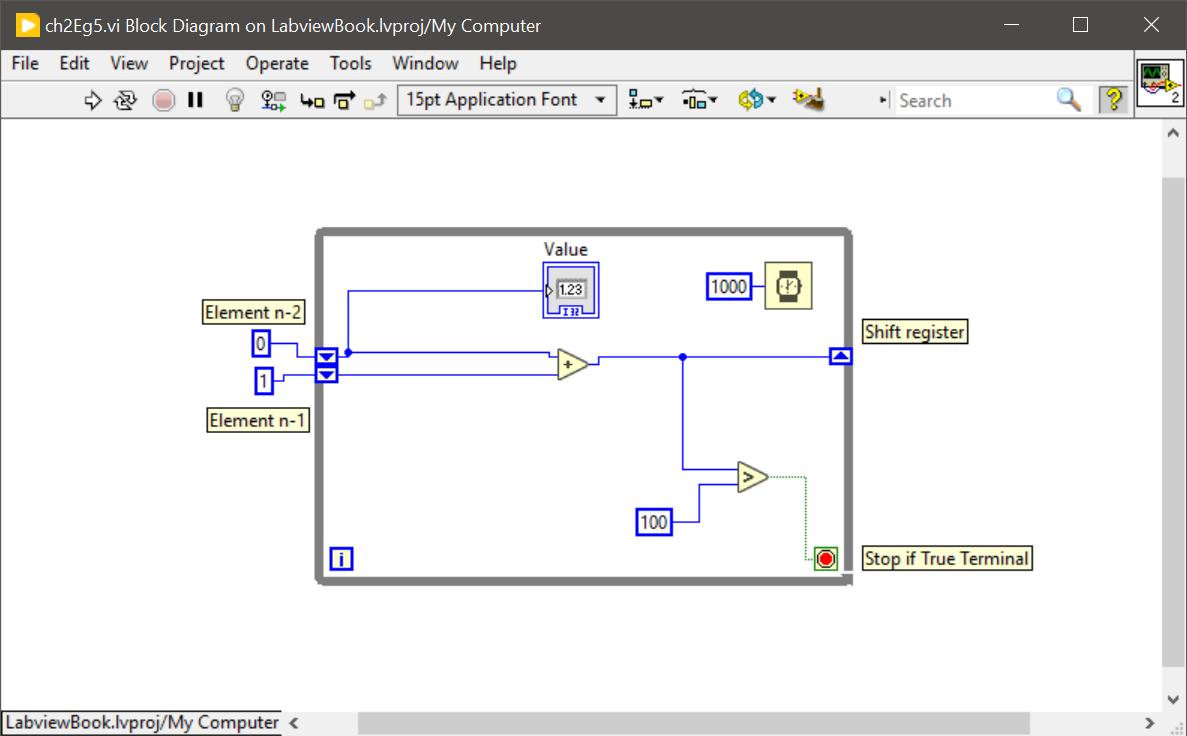
\includegraphics[width=\textwidth]{ch2eg5}
	\caption{A loop that displays the Fibonacci numbers less than 100, updating every second.}
	\label{ch2eg5}
\end{figure}

In this example, if a number in the sequence is greater than $100$, the comparison function sends a ``true'' value to the condition terminal which causes the loop to terminate. If this is slightly confusing, just remember ``Red means stop!.\\

If you \texttt{right click} on the condition terminal, you may change it to a ``Continue if true'' condition. In this case, the while loop will only terminate when it receives a ``false'' value. Conveniently, the terminal changes to a green circular arrow, in other words ``Green means go!. Figure \ref{whileCond} shows the two available condition types side by side. Yes that is a little octagon stop sign, it took me almost 5 years to notice that.\\
\begin{figure} %TODO Fix the condition figures to be the same size
	\centering
	\begin{subfigure}[b]{0.40\textwidth}
		\centering
		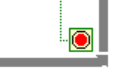
\includegraphics[width=\textwidth]{stopIfTrue}
		\caption{The ``stop if true'' while loop condition terminal.}
	\end{subfigure}
	\hfil
	\begin{subfigure}[b]{0.40\textwidth}
		\centering
		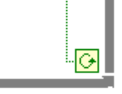
\includegraphics[width=\textwidth]{contIfTrue}
		\caption{The ``continue if true'' while loop condition terminal}
	\end{subfigure}
	\caption{The two available while loop conditions, also notice how the edge of the frame makes a little arrow.}
	\label{whileCond}
\end{figure}

Much like in other programming languages, infinite loops are considered unwanted behaviour. While loops must have their conditional terminals wired, even if your program would run for days or weeks on end, it should have a button to safely exit its execution. This will become more apparent in Chapter 3 where we will be programming hardware, other than your computer that is.\\

\section{Aggregate data types}
From here on out, the training wheels are off. The concept of an array is simple, the explanation in section \ref{ch1Arrays} is as detailed as needed and will not be repeated here. Working with arrays in $\labview$ is tricky however, in the next few pages we will dissect this creature and reveal some of the more ugly sides to this programming language.\\

\subsection{Arrays}
\subsubsection{Creation}
Technically an array is also a type of structure in $\labview$. In the block diagram view, a placed array constant contains nothing, not even a type. You provide the type by placing a constant inside the array box. This is seen preformed in figure \ref{createNumArrayConst}. In this particular case, an integer constant creates an empty integer array, seen in figure \ref{numArrayConst}.\\
\begin{figure} %TODO Fix the condition figures to be the same size
	\centering
	\begin{subfigure}[b]{0.40\textwidth}
		\centering
		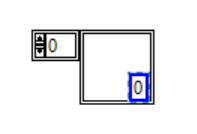
\includegraphics[width=\textwidth]{createNumArrayConst}
		\caption{An empty array constant, the integer constant has not been placed yet.}
		\label{createNumArrayConst}
	\end{subfigure}
	\hfil
	\begin{subfigure}[b]{0.40\textwidth}
		\centering
		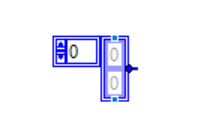
\includegraphics[width=\textwidth]{numArrayConst}
		\caption{An empty integer array constant, expanded to show two elements.}
		\label{numArrayConst}
	\end{subfigure}
	\caption{Creating an array constant.}
	\label{arrayConsts}
\end{figure}

The two little blue terminals in figure \ref{numArrayConst} are drag points to change the amount of visible elements in the array. Even if only one element is shown, you may cycle through the array using the arrows next to the $0$ seen in the figures. This $0$ corresponds to the index of the top visible element in the array. Array controls are made in a similar fashion on the front panel. Once you have made an array, you can start adding values. You do this by clicking on the grey $0$ and typing in a number.  

\subsubsection{Manipulation}
Figure \ref{ch2SimpleArrayBlock} shows how the numeric functions may be used to operate on arrays. These operations are preformed on an element by element basis. Figure \ref{ch2SimpleArrayFront} shows the result of these two operations. The result is truncated to the size of the smallest array.\\
\begin{figure}
	\centering
	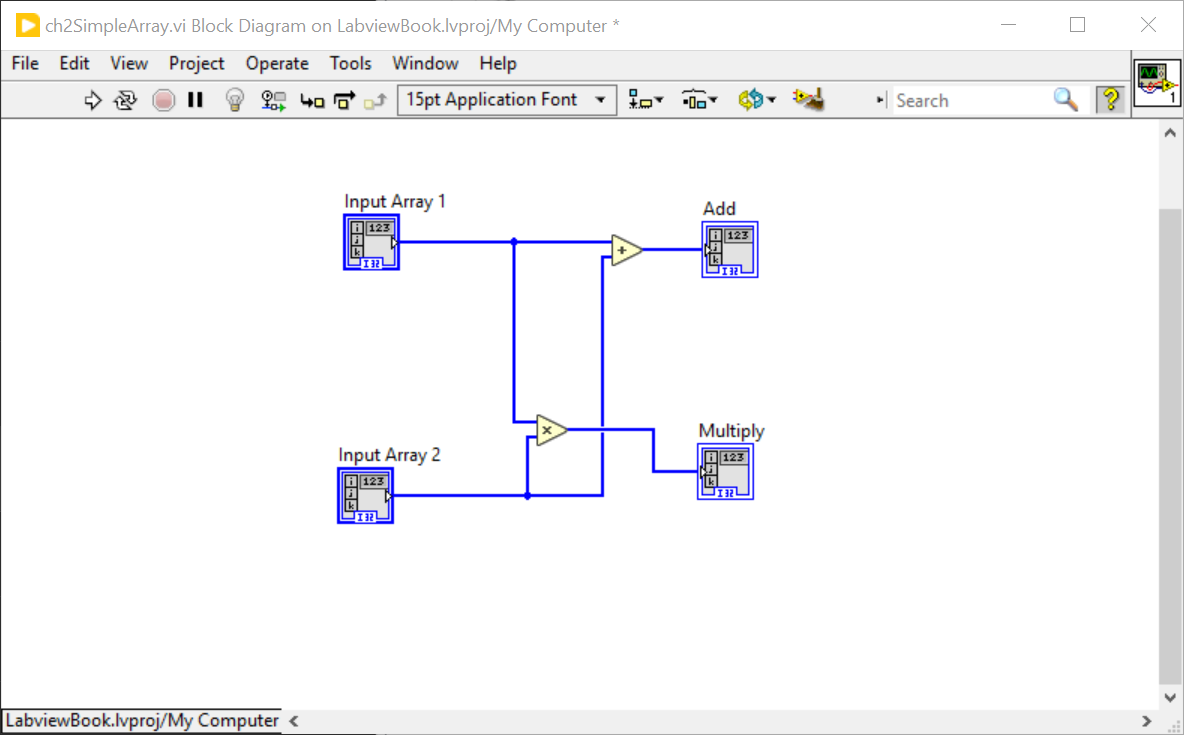
\includegraphics[width=\textwidth]{ch2SimpleArrayBlock}
	\caption{Two operations on array variables, these are the normal functions found in the ``Numeric'' folder in the functions palette.}
	\label{ch2SimpleArrayBlock}
\end{figure}
\begin{figure}
	\centering
	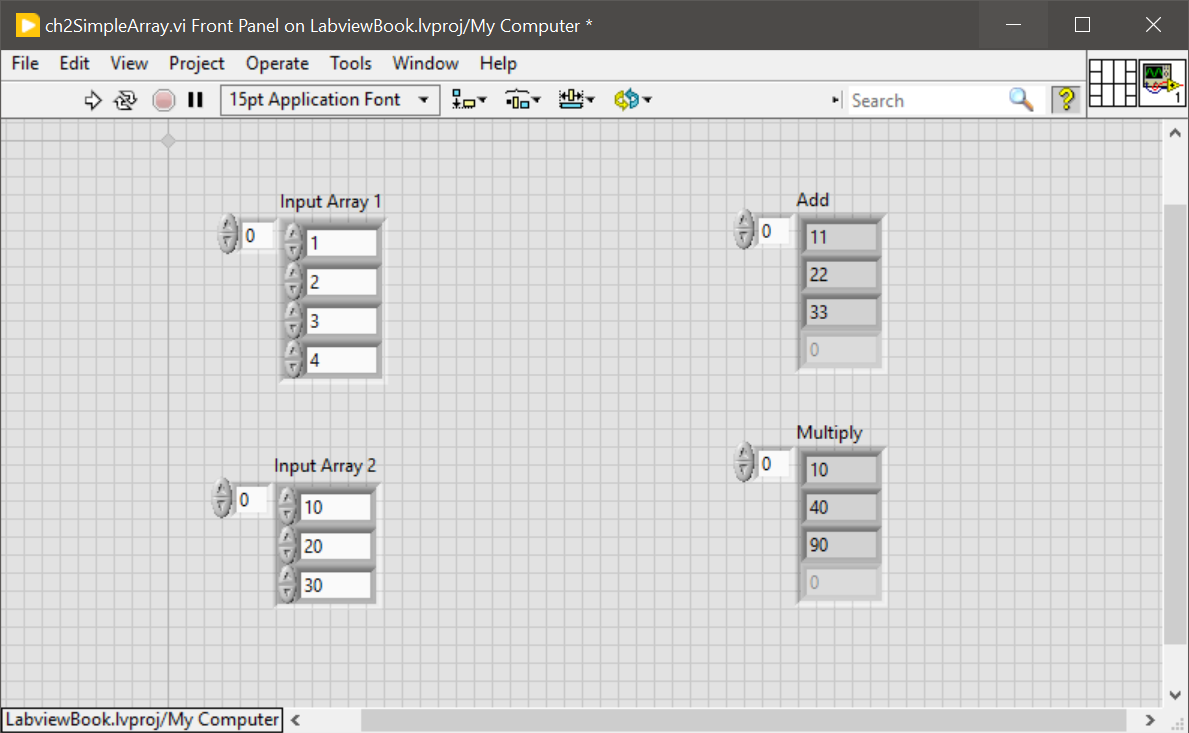
\includegraphics[width=\textwidth]{ch2SimpleArrayFront}
	\caption{The results of elementary operations on arrays.}
	\label{ch2SimpleArrayFront}
\end{figure}

There are also a few array specific functions in the numeric palette which yield the sum of all the array elements or the product all the elements. You should experiment with these on your own.\\

\subsubsection{Exploitation}
The real power, and complexity, of arrays emerge when operating on the elements themselves. Figure \ref{ch2IndexArrayBlock} shows some of the most important operations able to be performed on arrays.\\
\begin{figure}
	\centering
	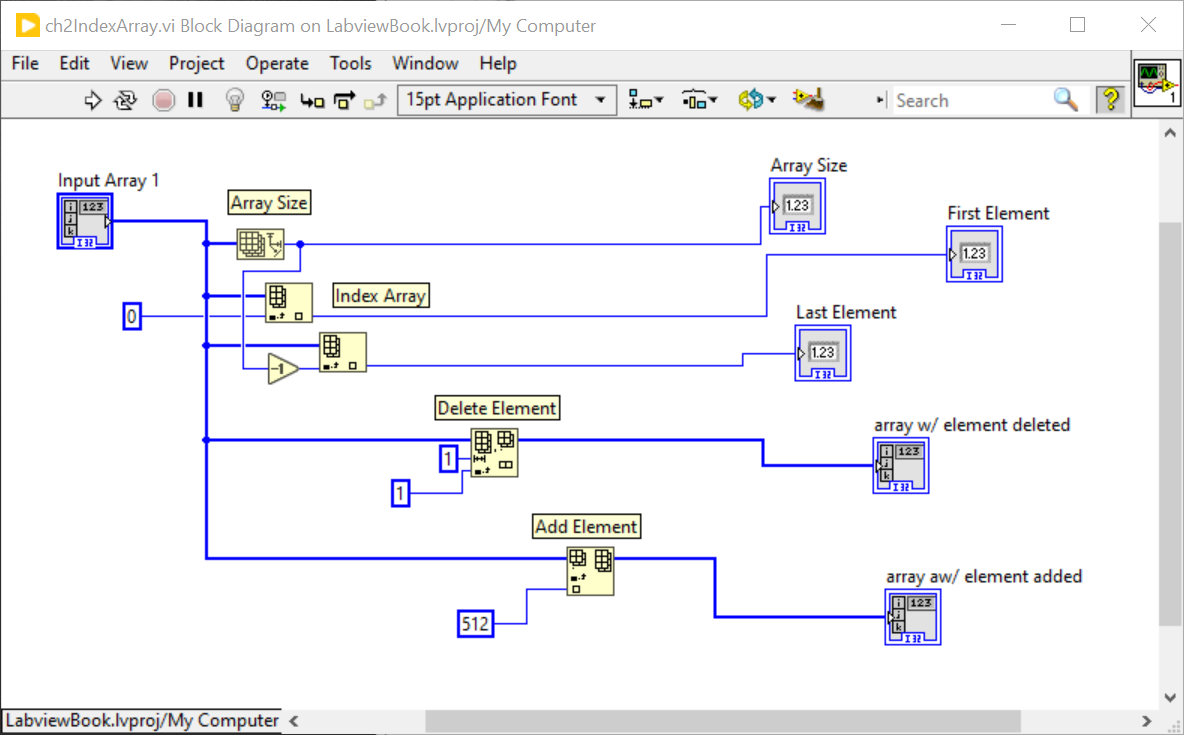
\includegraphics[width=\textwidth]{ch2IndexArrayBlock}
	\caption{Fundamental operations on arrays.}
	\label{ch2IndexArrayBlock}
\end{figure}

The array size function is rather self explanatory, it just gives you the number of elements in the array.\\

The index array function picks out an element of an array at the index you specified. Index $0$ being the first element in an array. Getting the last element of an array requires you to know its size, since indexing starts at $0$, you need to decrement the size before sending it to the index function.\\

Unlike in \texttt{C} programming, indexing an array out of bounds in $\labview$ will not destroy your computer. For numeric arrays, the index function will return $0$ upon indexing an out of range value and will continue with your program as if nothing has happened. Soon enough you will discover on your own what an ``off by one'' error is.\\

The delete array element function takes two arguments, an index value and length. This deletes the value at the selected index. If the length is more than one, the selected index and subsequent indexes are deleted. What do you think happens when you wire in a negative length value?\\ %TODO Test this, I don't know.

The add array element function adds an element into the index you specify, think of it like cutting in line at the bank. If you cut in line at position three from the front desk, the person behind you is now fourth and you are now third. I do not condone this behaviour, please exercise this in a computer program and not in real life.\\

Figure \ref{ch2IndexArrayFront} shows the results of these operations. The next step is to put these functions into context so you can see how they are used in more useful programs.\\
\begin{figure}
	\centering
	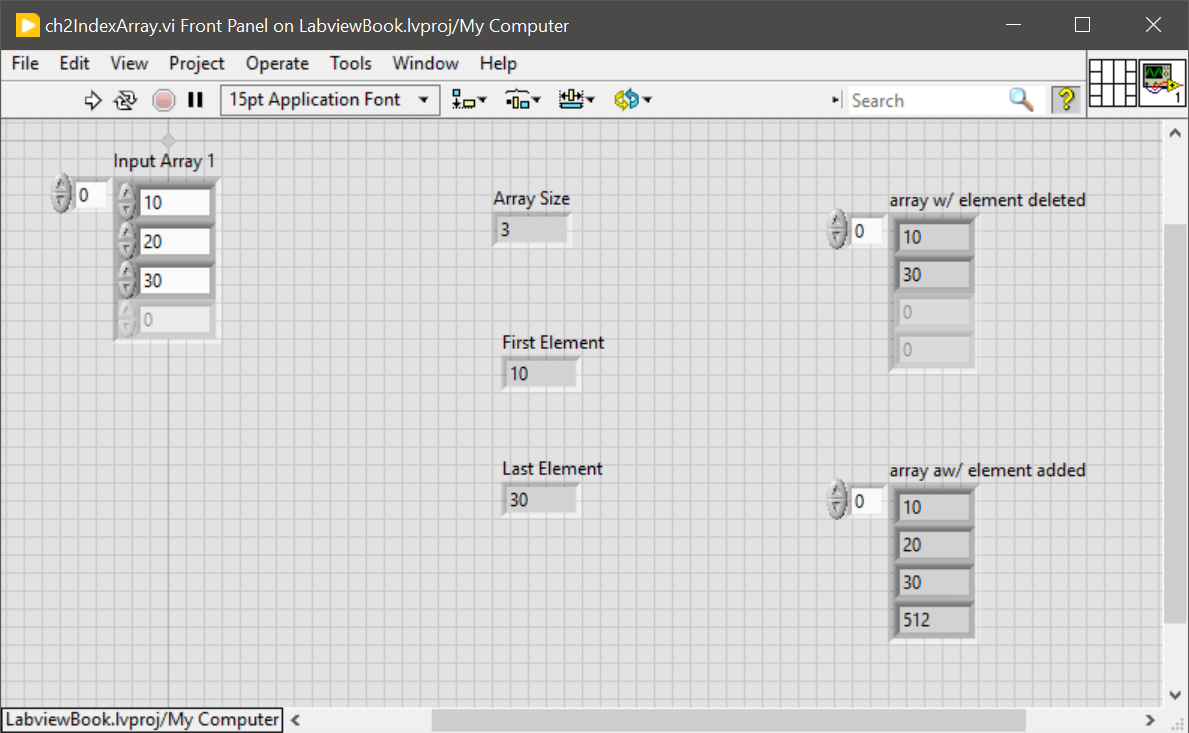
\includegraphics[width=\textwidth]{ch2IndexArrayFront}
	\caption{The results of fundamental operations on arrays.}
	\label{ch2IndexArrayFront}
\end{figure}

\subsubsection{Using arrays with loops}
\begin{figure}
	\centering
	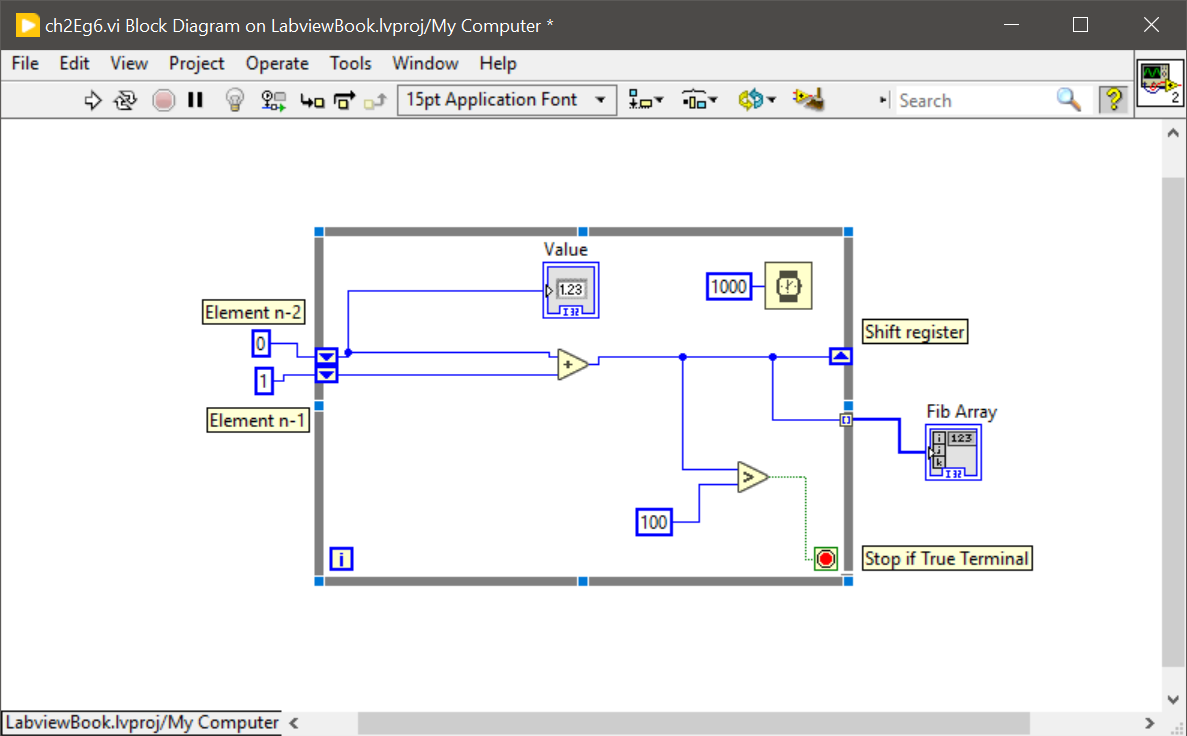
\includegraphics[width=\textwidth]{ch2eg6Block}
	\caption{Using auto indexing tunnels to create an array.}
	\label{ch2eg6Block}
\end{figure}
\begin{figure}
	\centering
	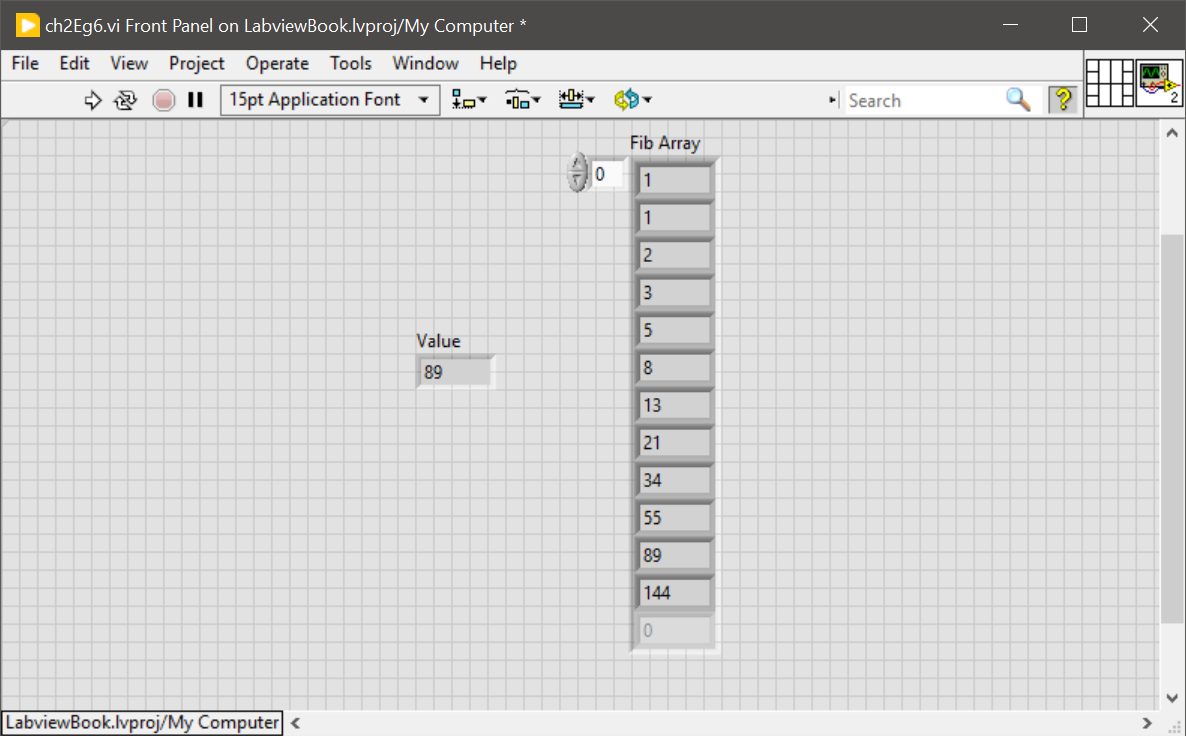
\includegraphics[width=\textwidth]{ch2eg6Front}
	\caption{The output of an auto indexing tunnel, do you notice what is wrong here?}
	\label{ch2eg6Front}
\end{figure}


\begin{figure}
	\centering
	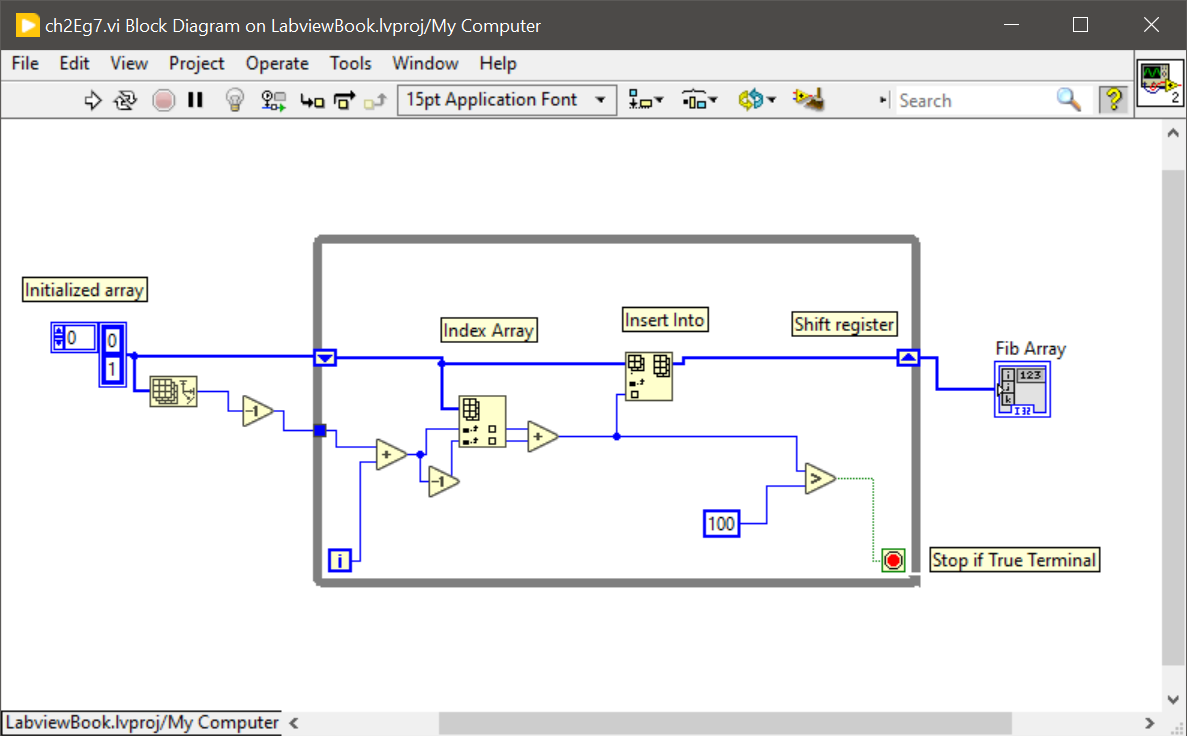
\includegraphics[width=\textwidth]{ch2eg7}
	\caption{A rewrite of the program that gives the expected results.}
	\label{ch2eg7}
\end{figure}
\section{Creating functions}

\section{Slightly more advanced Mini Projects}